\subsection{Ртутная лампа}
Построим график $d_i^2 = F(i)$ для зелёной линии ртути, приняв 
длину её волны $\lambda (Hg) = 5461$ \AA. По наклону 
полученной прямой рассчитаем базу $L$ интерферометра, используя 
формулу 
\begin{equation}\label{eq::A_2}
  \frac{\lambda}{L} = \frac{1}{4f^2} \frac{\Delta(d_i)}{\Delta(i)}
\end{equation}


\import{./}{hg_green_circ.tex}
По полученным данным построим график:

\begin{figure}[h]
  \center{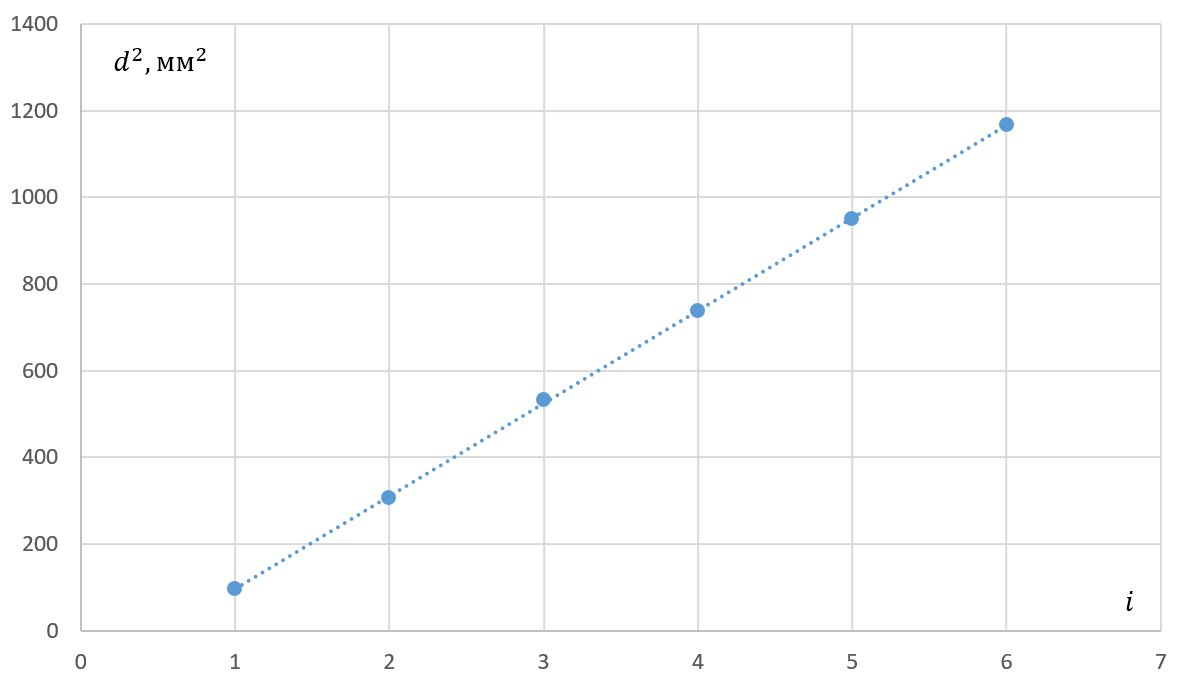
\includegraphics[width=0.7\linewidth]{graph_hg_d_from_i.png}}
  \caption{График зависимости $d_i^2$ от $i$}
  \label{img::gr_1}
\end{figure}

С помощью метода наименьших квадратов найдём коэффициент наклона этой 
прямой, откуда по формуле \eqref{eq::A_2}:
$$
L = (1.17 \pm 0.01) \cdot 10^{-1} мм.
$$

Рассчитаем средние диаметры $\overline{d}$ для жёлтых пар колец
$Hg$ и разности этих диаметров $\Delta d$ для колец одного порядка.

\import{./}{hg_yellow_circ.tex}

По полученным данным построим график 
\begin{figure}[h]
  \center{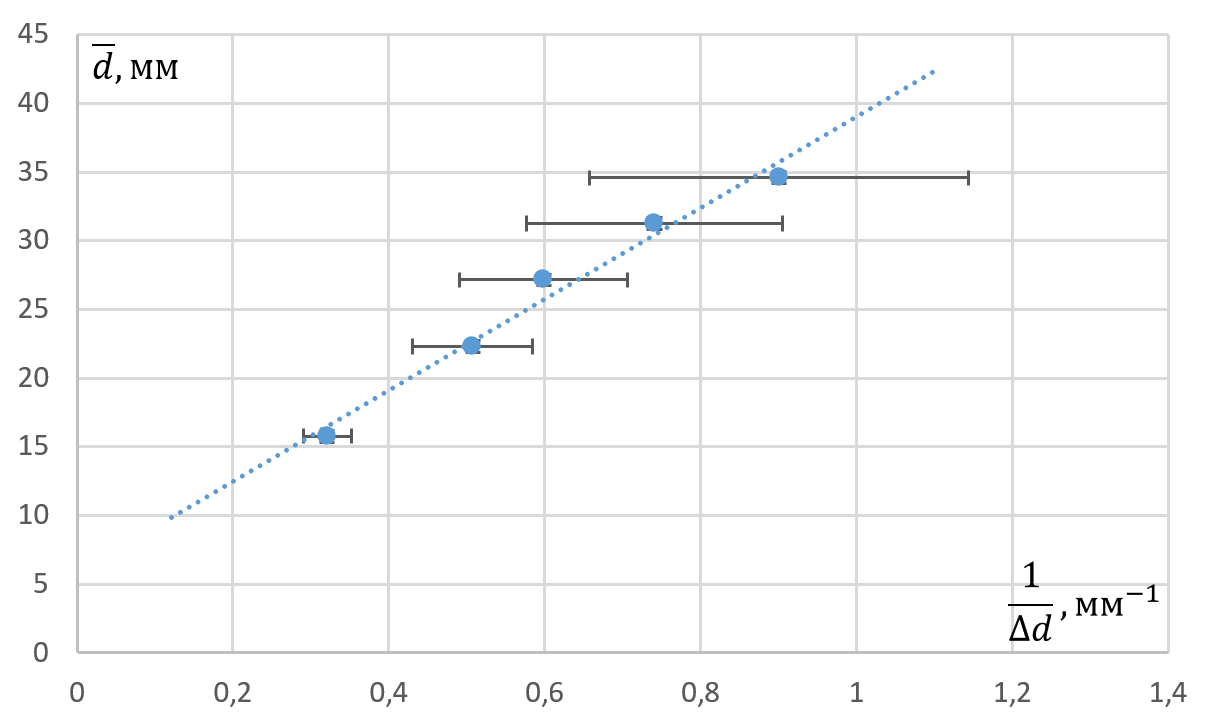
\includegraphics[width=0.8\linewidth]{graph_hg_avd_delta.png}}
  \caption{График зависимости $\overline{d}$ от $\frac{1}{\Delta d}$}
\end{figure}

По углу наклона прямой полученного графика рассчитаем разность
длин волн для жёлтой пары линий ртути:
$$
\Delta \lambda = 3.9 \pm 0.3 \text{\: \AA}
$$

\newpage
\subsection{Натриевая лампа}

Построим график $d_i^2 = F(i)$ для одной из линий дуплета натрия, приняв 
длину волны $\lambda (Hg) = 5893$ \AA. По наклону 
полученной прямой рассчитаем базу $L$ интерферометра, используя 
формулу 
\begin{equation}\label{eq::A_3_2}
  \frac{\lambda}{L} = \frac{1}{4f^2} \frac{\Delta(d_i)}{\Delta(i)}
\end{equation}


\begin{table}[h]
  \caption{Измерение диаметров жёлтых колец для $Na$}
  \begin{center}
    \import{./}{na.tex}
  \end{center}
\end{table}
По полученным данным построим график:

\begin{figure}[h!]
  \center{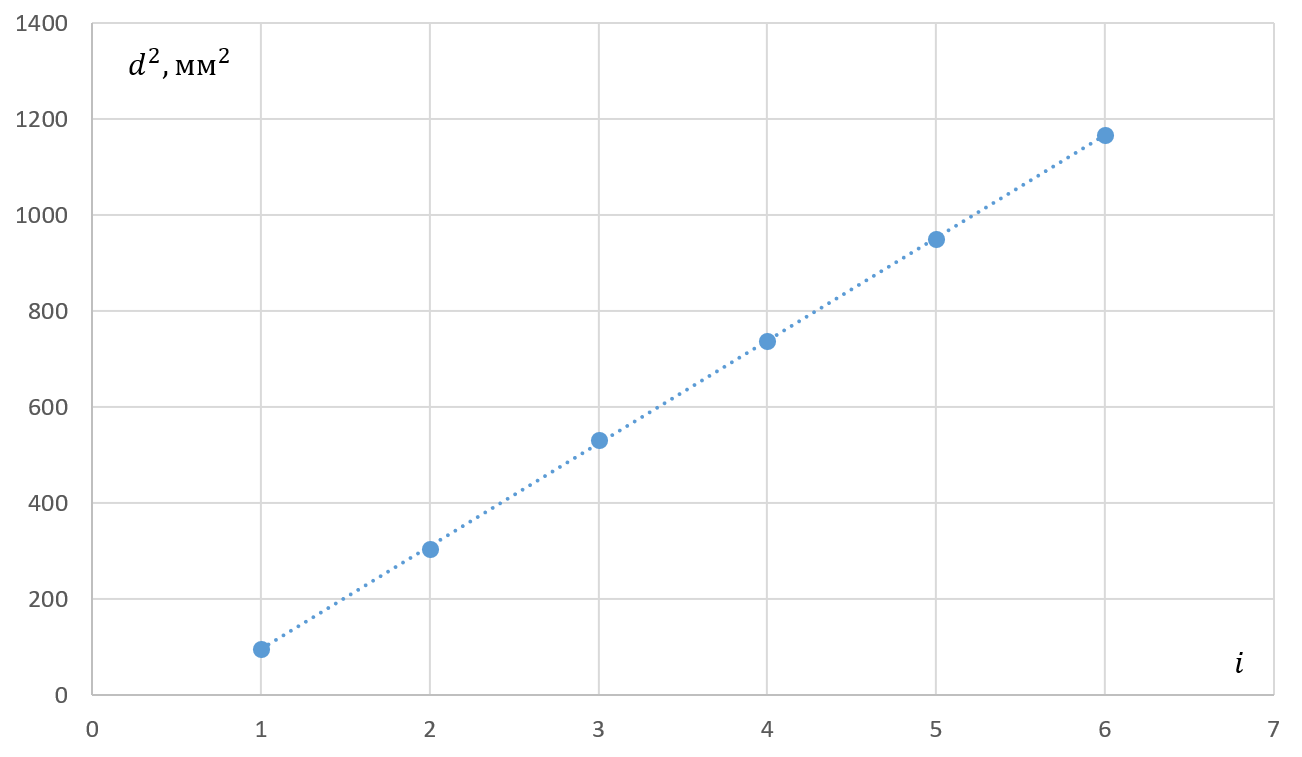
\includegraphics[width=0.7\linewidth]{graph_na_d_from_i.png}}
  \caption{График зависимости $d_i^2$ от $i$}
  \label{img::gr_1}
\end{figure}

С помощью метода наименьших квадратов найдём коэффициент наклона этой 
прямой, откуда по формуле \eqref{eq::A_3_2}:
$$
L = (9.73 \pm 0.11) \cdot 10^{-2} мм.
$$

Рассчитаем средние диаметры $\overline{d}$ для жёлтых пар колец
$Na$ и разности этих диаметров $\Delta d$ для колец одного порядка.

\begin{table}[h]
  \caption{К рассчёту $\overline{d}$ и $\frac{1}{\Delta d}$}
  \center{
\begin{tabular}{| c | c | c | c | c |}
  \hline
  $i$ & $\overline{d}$, мм & $\sigma_{\overline{d}}$, мм & $\frac{1}{\Delta_d}, \text{мм}^{-1}$ & $\sigma, \text{мм}^{-1}$\\
  \hline
  $1$ & $7,32$ & $3 \cdot 10^{-2}$ & $0,20$ & $0,002$ \\
  \hline
  $2$ & $16,60$ & $3 \cdot 10^{-2}$ & $0,57$ & $0,02$ \\
  \hline
  $3$ & $22,27$ & $3 \cdot 10^{-2}$ & $0,64$ & $0,02$ \\
  \hline
  $4$ & $26,60$ & $3 \cdot 10^{-2}$ & $0,86$ & $0,04$ \\
  \hline
  $5$ & $30,29$ & $3 \cdot 10^{-2}$ & $0,90$ & $0,05$ \\
  \hline
  $6$ & $33,63$ & $3 \cdot 10^{-2}$ & $0,97$ & $0,06$ \\
  \hline
\end{tabular}
  }
\end{table}

По полученным данным построим график 
\begin{figure}[h]
  \center{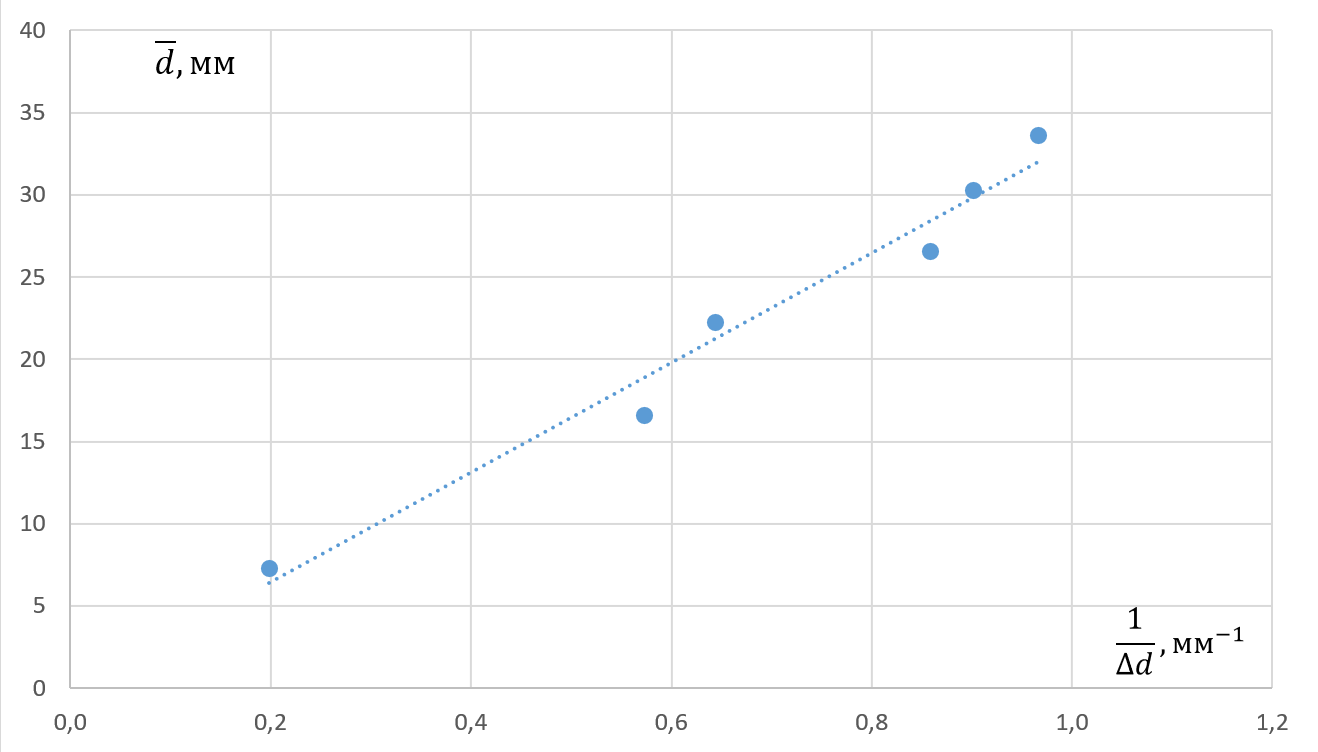
\includegraphics[width=0.8\linewidth]{graph_na_avd_delta.png}}
  \caption{График зависимости $\overline{d}$ от $\frac{1}{\Delta d}$}
\end{figure}

По углу наклона прямой полученного графика рассчитаем разность
длин волн для жёлтой пары линий натрия:
$$
\Delta \lambda = 5.6 \pm 0.4 \text{\: \AA}
$$

\subsection{Общие расчёты}

Используя разность диаметров и разность длин волн жёлтых пар 
$Na$ и $Hg$ оценим экспериментальные значения линейной 
дисперсии интерферометров:

\begin{table}[h]
  \caption{Сравение теории и эксперимента для $Na$}
  \center{\import{./}{NaDD.tex}}
\end{table}

\import{./}{hgDD.tex}

Оценим также аппаратную разрешающую способность по формуле:
$$
R_{апп} = \frac{\lambda}{\delta \lambda} 
\simeq
\frac{1}{\Theta \cdot \delta \Theta}
\simeq
\frac{4f^2}{d\cdot\delta r}
$$

Откуда получим для $Hg$ и $Na$:
$$
R_{апп}^{Na} = 
(5.06 \pm 0.05) \cdot 10^3, \: \: 
R_{апп}^{Hg} = 
(7.10 \pm 0.05) \cdot 10^3
$$

Оценим число максимумов $m_{Na} \approx \frac{2L}{\lambda}
= 340$, откуда число интерферирующих полос $N = \frac{R^{Na}}{m_{Na}} \approx 15$.

Приняв коэффициент отражения $r \simeq 0.85$, получим для добротности:
$$
Q =   \frac{\pi\sqrt{r}}{1-r}m \approx 6500
$$